%======================================================================
% NewsAnalyzer Ubi-Media 2027 Submission Template (LLNCS)
% Grounded Real-Time Fake News Detection on Traditional Chinese Social Media
% via Macro Fact-Checking Census and Multi-Signal Metadata Fusion
%======================================================================

\documentclass[twoside]{llncs}
\usepackage[utf8]{inputenc}
\usepackage[T1]{fontenc}
\usepackage{upquote}
\usepackage{listings}
\usepackage[english]{babel}
\usepackage{url}
\usepackage{xurl}
\usepackage[hidelinks]{hyperref}
\usepackage{graphicx}
\usepackage{amsmath,amssymb}
\usepackage{booktabs}
\usepackage[expansion=false]{microtype}
\usepackage{float}
\usepackage{cite}
\usepackage{tikz}
\usetikzlibrary{arrows.meta, positioning}
\setlength{\textfloatsep}{8pt plus 2pt minus 2pt}
\setlength{\floatsep}{6pt plus 2pt minus 2pt}
\setlength{\intextsep}{6pt plus 2pt minus 2pt}

%======================================================================
% TITLE / AUTHOR
%======================================================================
\title{NewsAnalyzer: Real-Time Fake News Detection on Social Media\texorpdfstring{\\ \vspace{0.5em}\large}{ - }via Multi-Signal Metadata Fusion and Local Semantic Verification}
\titlerunning{NewsAnalyzer: Multi-Signal Fake News Detection on Social Media}
\authorrunning{T. Lin, H. Lin, and S.-C. Chen}

\author{Tsangyu Lin\inst{1} \and Hui Lin\inst{1}\thanks{Corresponding author.} \and Sheng-Chih Chen\inst{2}}

\institute{
Department of Computer Science and Information Engineering, \\
Tamkang University, New Taipei City 25137, Taiwan \\
\email{jefflin.je598@gmail.com, 121678@mail.tku.edu.tw}
\and
National Chengchi University, Taipei, Taiwan \\
\email{scchen@nccu.edu.tw}}

\begin{document}

\maketitle

%======================================================================
% ABSTRACT
%======================================================================
\begin{abstract}
Fake news spreads fast on Traditional Chinese social media like Facebook, LINE chats, and Threads. Real news and fake posts look the same in the feed, so readers cannot tell them apart. Large language models are poor judges for this job: they do not know new hoaxes, they believe smooth but fake writing, and they give scores with no proof behind them. Cloud APIs are also slow and send user data away. Therefore, this study builds \textbf{NewsAnalyzer}, a checker that ties every score to proof it actually found. It has three parts: (1) a local list of $N=2{,}292$ checked claims from Cofacts with SBERT search, (2) scores for website trust, feeling words, and how new a post is, and (3) a hard cap at 25 points ($S \le 25$) whenever proof against the claim is found. A local Qwen3.8-27B model only writes short summaries and never makes the call. We tested all 2,292 claims with 5-fold cross-validation under rewrites from light to heavy. The checker was right 95.3\% of the time ($F_1 = 0.974$) on solved claims and answers in 1.48\,ms. Against majority, TF-IDF, NewsGuard-style, and plain-LLM baselines, it was more accurate while keeping all user data on the user's own machine.
\keywords{Fake news detection, Traditional Chinese social media, fact-checking census, metadata scoring, semantic retrieval, dynamic safety anchoring, edge inference.}
\end{abstract}

%======================================================================
% 1 INTRODUCTION
%======================================================================
\section{Introduction}

In Taiwan, digital news consumption is heavily concentrated within high-velocity social platforms such as Facebook, LINE group chats, and Threads. In these environments, legitimate news reporting, hyperpartisan commentary, deceptive content-farm clickbait, and unverified public health rumors circulate in identical visual formats, often separated by only a single scroll. Combating this infodemic directly at the point of consumption requires credibility assessments that are accurate, instantly accessible, and strictly protective of user browsing privacy.

Recent academic and commercial initiatives have increasingly turned to standalone Large Language Models (LLMs) as zero-shot truth arbiters. However, relying on brute-force LLM generation as the primary judge introduces critical structural failure modes:
\begin{enumerate}
  \item \textbf{Temporal Blindness and Information Lag}: Pre-trained LLM weights reflect a historical knowledge cutoff and cannot reliably evaluate breaking rumors or localized viral hoaxes that emerged hours or days prior.
  \item \textbf{Susceptibility to Stylistic Deception}: As generative AI tools lower the cost of producing polished propaganda, modern misinformation frequently exhibits formal syntax and authoritative phrasing. Unconstrained LLMs evaluate such text as plausible and credible due to its fluent surface structure.
  \item \textbf{Absence of Auditable Provenance}: Brute-force LLMs output subjective score predictions without binding them to verified investigation archives, risking plausible-sounding hallucinations that undermine user trust.
  \item \textbf{Latency and Privacy Penalties}: Dispatching live browser DOM contents and browsing history to third-party cloud LLM APIs incurs severe round-trip latencies (5--10\,s) and creates significant privacy vulnerabilities.
\end{enumerate}

\begin{figure}[!htbp]
\centering
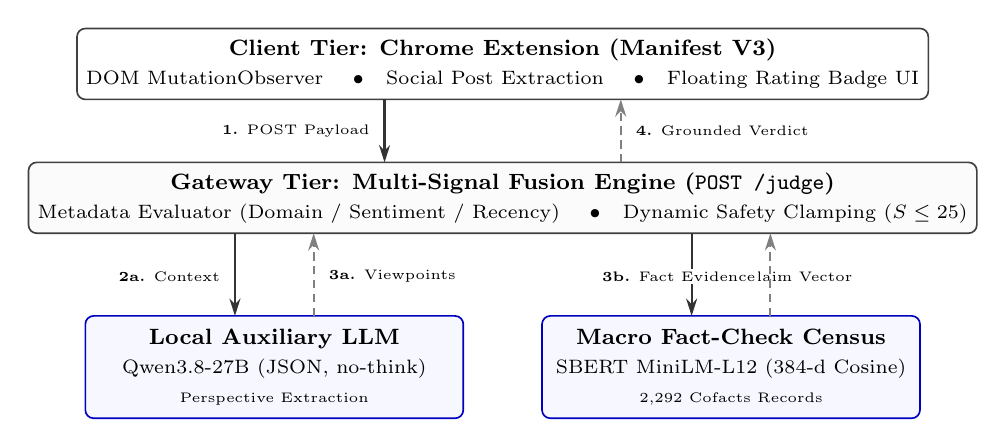
\begin{tikzpicture}[
  box/.style={draw=black!75, rounded corners=3pt, fill=white, align=center,
              font=\footnotesize, line width=0.6pt},
  srv/.style={draw=black!75, rounded corners=3pt, fill=gray!3, align=center,
              font=\footnotesize, line width=0.6pt},
  eng/.style={draw=blue!75!black, rounded corners=3pt, fill=blue!3, align=center,
              font=\footnotesize, line width=0.6pt},
  arr/.style={-{Stealth[length=2.2mm, width=1.4mm]}, thick, draw=black!80},
  revarr/.style={-{Stealth[length=2.2mm, width=1.4mm]}, thick, draw=black!50,
                 densely dashed},
  lbl/.style={font=\tiny, fill=white, inner sep=1pt}
]

  % ========== TIER 1: Client ==========
  \node[box, minimum width=10.4cm, minimum height=0.9cm] (t1) at (0, 3.3) {
    \textbf{Client Tier: Chrome Extension (Manifest V3)}\\[1pt]
    \scriptsize DOM MutationObserver \quad$\bullet$\quad
    Social Post Extraction \quad$\bullet$\quad
    Floating Rating Badge UI
  };

  % ========== TIER 2: Gateway ==========
  \node[srv, minimum width=10.4cm, minimum height=0.9cm] (t2) at (0, 1.6) {
    \textbf{Gateway Tier: Multi-Signal Fusion Engine (\texttt{POST /judge})}\\[1pt]
    \scriptsize Metadata Evaluator (Domain / Sentiment / Recency) \quad$\bullet$\quad
    Dynamic Safety Clamping ($S \le 25$)
  };

  % ========== TIER 3: Dual Cores ==========
  \node[eng, minimum width=4.8cm, minimum height=1.3cm] (qwenllm) at (-2.9, -0.55) {
    \textbf{Local Auxiliary LLM}\\[1pt]
    \scriptsize Qwen3.8-27B (JSON, no-think)\\[1pt]
    \tiny Perspective Extraction
  };

  \node[eng, minimum width=4.8cm, minimum height=1.3cm] (sbert) at (2.9, -0.55) {
    \textbf{Macro Fact-Check Census}\\[1pt]
    \scriptsize SBERT MiniLM-L12 (384-d Cosine)\\[1pt]
    \tiny 2,292 Cofacts Records
  };

  % ======== ARROWS: T1 <-> T2 ========
  \draw[arr] (-1.5, 2.85) -- (-1.5, 2.05);
  \node[lbl, anchor=east] at (-1.65, 2.45)
    {\textbf{1.} POST Payload};

  \draw[revarr] (1.5, 2.05) -- (1.5, 2.85);
  \node[lbl, anchor=west] at (1.65, 2.45)
    {\textbf{4.} Grounded Verdict};

  % ======== ARROWS: T2 <-> QWEN ========
  \draw[arr] (-3.4, 1.15) -- (-3.4, 0.1);
  \node[lbl, anchor=east] at (-3.55, 0.6)
    {\textbf{2a.} Context};

  \draw[revarr] (-2.4, 0.1) -- (-2.4, 1.15);
  \node[lbl, anchor=west] at (-2.25, 0.6)
    {\textbf{3a.} Viewpoints};

  % ======== ARROWS: T2 <-> SBERT ========
  \draw[arr] (2.4, 1.15) -- (2.4, 0.1);
  \node[lbl, anchor=west] at (2.55, 0.6)
    {\textbf{2b.} Claim Vector};

  \draw[revarr] (3.4, 0.1) -- (3.4, 1.15);
  \node[lbl, anchor=east] at (3.25, 0.6)
    {\textbf{3b.} Fact Evidence};

\end{tikzpicture}
\caption{Layered architecture of NewsAnalyzer: the client extension extracts live social DOM elements and communicates with the local gateway, which prioritizes empirical fact-check census retrieval and multi-signal metadata evaluation, utilizing an auxiliary local LLM only for structured viewpoint extraction.}
\label{fig:arch}
\end{figure}

To overcome these structural limitations, we introduce \textbf{NewsAnalyzer}, a grounded multi-signal verification framework tailored to Traditional Chinese social media. Rather than treating an LLM as an ungrounded oracle, NewsAnalyzer anchors its detection pipeline on an offline macro census of verified fact-checking records ($N=2{,}292$) sourced from the collaborative Cofacts repository and accredited by the International Fact-Checking Network (IFCN). This empirical base is fused with rich metadata heuristics (domain reputation, sentiment volatility, clickbait valence, and temporal decay) and enforced by an asymmetric safety clamping mechanism that overrules speculative model generation when verified counter-evidence exists. An on-device auxiliary LLM (Qwen3.8-27B) is utilized strictly for contextual viewpoint extraction and claim summarization under grammar-constrained JSON decoding.

The main contributions of this work are:
\begin{itemize}\setlength{\itemsep}{2pt}
  \item \textbf{Deconstruction of Brute-Force LLM Limitations}: We formulate the systemic failure modes of standalone zero-shot LLMs in regional social environments, showing why empirical grounding and multi-signal metadata are necessary prerequisites for reliable verification.
  \item \textbf{Macro Fact-Check Census and Sub-2\,ms Retrieval}: We construct an offline semantic index over 2,292 IFCN-verified claims from the localized Cofacts archive, achieving 95.3\% accuracy ($F_1 = 0.974$), 99.9\% top-1 recall, and 1.48\,ms retrieval latency.
  \item \textbf{Multi-Signal Metadata Scoring and Dynamic Safety Anchoring}: We propose a composite scoring formulation combining domain blacklist heuristics, sentiment volatility, and temporal decay with an asymmetric clamp ($S \le 25$) that eliminates hallucinated false negatives on known hoaxes.
  \item \textbf{Privacy-Preserving Edge Architecture and Baseline Comparison}: We implement an open-source browser extension and local inference server, benchmarking its accuracy and resilience against pure zero-shot LLMs, surface NLP classifiers, and domain heuristics.
\end{itemize}

%======================================================================
% 2 RELATED WORKS
%======================================================================
\section{Related Works and Competing Paradigms}

Existing approaches to automated credibility assessment fall into three principal paradigms, each characterized by distinct operational trade-offs.

\subsection{Standalone and Brute-Force LLM Verification}
Recent studies have investigated prompt-based verification using general-purpose LLMs~\cite{guo2022survey, chern2023factool}. Frameworks such as FreshLLMs~\cite{vu2024freshllms} augment generation by querying external search engines dynamically during inference. While effective for open-domain English questions, real-time web querying introduces substantial latency (5--10\,s) that interrupts browser interaction. Moreover, standalone LLMs evaluated on Chinese social content struggle with nuanced local slang and frequently exhibit temporal blindness on recent political and health hoaxes. In contrast, NewsAnalyzer restricts the LLM to an auxiliary contextual summarizer, grounding all primary truth determinations in empirical fact-checking data.

\subsection{Surface NLP and Lexical Classifiers}
Early automated fake news detection relied on surface stylometrics, lexicon frequency analysis, and bag-of-words classifiers trained on benchmarks such as LIAR~\cite{wang2017liar, perez2018automatic, rashkin2017truth, potthast2018stylometric}. While computationally lightweight, these lexical models are brittle against paraphrased claims, rhetorical irony, and emerging online jargon. NewsAnalyzer moves beyond surface lexicons by pairing dense 384-dimensional Sentence-BERT~\cite{reimers2019sbert} embeddings with multi-attribute metadata heuristics.

\subsection{Domain-Level Reputation and Crowdsourced Fact-Checking}
Platform-level tools such as NewsGuard~\cite{Bianchi2024trustworthiness} evaluate publisher credibility at the domain level. While effective for flagging established content farms, domain heuristics fail completely on enclosed social platforms (e.g., Facebook and LINE), where credible journalism and malicious hoaxes share identical hostnames. Crowdsourced fact-checking repositories like Cofacts~\cite{cofacts2020, lim2023factchecking} collect volunteer refutations cross-referenced with accredited fact-checkers (Taiwan FactCheck Center~\cite{tfc2023}, MyGoPen). NewsAnalyzer leverages this civic data census as a local, offline vector database, bridging macro fact-checking intelligence directly into the client viewport.

%======================================================================
% 3 METHODOLOGY
%======================================================================
\section{Methodology}

NewsAnalyzer coordinates a client-side browser extension with a local multi-signal backend service. Figure~\ref{fig:arch} depicts the operational dataflow.

\subsection{Macro Fact-Check Census and Vector Space Indexing}
To establish an empirical ground truth for Traditional Chinese social rumors, we compile an offline index from the Cofacts open repository~\cite{cofacts2020, lim2023factchecking}. The local database contains $N=2{,}292$ verified claims that satisfy our length filter ($\text{length}(\text{text}) > 40$), partitioned into 1,817 \texttt{inaccurate}, 208 \texttt{partial}, and 267 \texttt{accurate} records cross-verified by IFCN-accredited organizations~\cite{ifcn2020, tfc2023}.

We deploy a multilingual Sentence-BERT model~\cite{reimers2019sbert} (MiniLM-L12) executing entirely on the host CPU. Claim vectors are stored in a compressed memory-mapped array (\texttt{sbert\_index.npz}, shape $2292 \times 384$). When a candidate post is ingested from the DOM, the server projects its text into vector space $\mathbf{q} \in \mathbb{R}^{384}$ and evaluates cosine similarity against all indexed claim vectors $\mathbf{d}_i$:
\begin{equation}
\text{sim}(\mathbf{q}, \mathbf{d}_i) = \frac{\mathbf{q} \cdot \mathbf{d}_i}{\|\mathbf{q}\| \|\mathbf{d}_i\|}
\end{equation}
The system retrieves the top-$k$ ($k=5$) candidates. If the maximal similarity exceeds the empirical evidence threshold $\theta_{\text{sim}} = 0.72$, the system retrieves the verified record as direct factual evidence (\texttt{fc\_hit} is true); otherwise, the status defaults to \texttt{not\_found}.

\subsection{Multi-Signal Metadata Scoring Engine}
Rather than relying on isolated text classifications, NewsAnalyzer aggregates heterogeneous metadata indicators into a base heuristic score $S_{\text{base}} \in [0, 100]$:
\begin{enumerate}
  \item \textbf{Domain Reputation \& Blacklist ($M_{\text{dom}}$)}: Assigns positive credibility weights to recognized investigative news outlets, applies severe penalties to confirmed content farms listed in our local blacklist, and penalizes unencrypted HTTP origins.
  \item \textbf{Sentiment Volatility \& Clickbait Valence ($M_{\text{sent}}$)}: Evaluates emotional intensity and sensationalist phrasing using a distilled sentiment model to detect manipulative clickbait headlines.
  \item \textbf{Temporal Decay ($M_{\text{time}}$)}: Applies exponential decay penalties to stale, unverified historical claims that resurface out of context.
  \item \textbf{Crowdsourced Signal ($M_{\text{crowd}}$)}: Integrates community report frequencies and consensus metrics when available.
\end{enumerate}

\subsection{Dynamic LLM Fusion and Asymmetric Safety Clamping}
When the auxiliary local LLM produces a generative credibility score $S_{\text{LLM}} \in [0, 100]$, the gateway dynamically fuses it with the metadata score:
\begin{equation}
S_{\text{fused}} = (1 - w_{\text{fusion}}) \cdot S_{\text{base}} + w_{\text{fusion}} \cdot S_{\text{LLM}}
\end{equation}
The fusion weight $w_{\text{fusion}}$ adapts according to the retrieval state:
\begin{equation}
w_{\text{fusion}} = 
\begin{cases}
0.10, & \text{if verified Cofacts evidence is retrieved (\texttt{fc\_hit} is true)} \\
0.60, & \text{if no fact-checking record matches (\texttt{fc\_hit} is false)}
\end{cases}
\end{equation}
This formulation ensures that verified fact-checking records dominate the final verdict, while LLM reasoning is given primary analytical weight only when empirical evidence is absent.

\subsubsection{Asymmetric Safety Anchor Clamping}
To prevent fluent LLM hallucinations from overriding known malicious rumors, the system enforces a non-linear safety clamp:
\begin{equation}
S_{\text{final}} =
\begin{cases}
\min(S_{\text{fused}}, 25.0), & \text{if status } \in \{\texttt{inaccurate}, \texttt{false}\}, \text{ sim} \ge 0.85 \\
\min(S_{\text{fused}}, 50.0), & \text{if status } \in \{\texttt{inaccurate}, \texttt{false}\}, 0.72 \le \text{sim} < 0.85 \\
\min(S_{\text{fused}}, 55.0), & \text{if status } \in \{\texttt{partial}\} \\
S_{\text{fused}}, & \text{otherwise}
\end{cases}
\end{equation}
This strict upper bound ($S \le 25.0$) ensures that even if an unconstrained prompt assigns high credibility to a well-written hoax, the confirmed empirical evidence strictly overrides the generative output.

\subsection{Auxiliary Local Contextual Analysis}
When invoked, Qwen3.8-27B~\cite{qwen2025report} executes locally via a llama.cpp server using 4-bit quantization (Q4\_K\_P)~\cite{gguf2023} with FastMTP speculative draft heads for accelerated decoding. To guarantee UI stability, we disable chain-of-thought reasoning and enforce grammar-constrained JSON decoding (\texttt{response\_format:\allowbreak json}), restricting generation strictly to four structured keys: factual summary (\texttt{key\_points}), opposing viewpoints (\texttt{viewpoints}, $<80$ chars), numeric rating (\texttt{credibility\_score}), and brief analysis (\texttt{analysis}, $<100$ chars).

\begin{lstlisting}[basicstyle=\ttfamily\tiny,breaklines=true,
  columns=fullflexible,keepspaces=true,showstringspaces=false,
  frame=single,framesep=2pt,aboveskip=2pt,belowskip=2pt]
SYSTEM: You are a Traditional Chinese fact-checking analyst. Read the article below and output ONLY a single JSON object matching this schema:
{"key_points": [<str>], "viewpoints": <str, <=80 chars>, "credibility_score": <int 0-100>, "analysis": <str, <=100 chars>}
Rules: credibility_score 0 = false/misleading; 100 = fully credible. Consider domain reputation, cited evidence, consistency, recency. NEVER add commentary outside JSON. NEVER emit markdown fences or <thought> tags. Output must parse with json.loads().
USER: <ARTICLE TITLE> \n <ARTICLE URL> \n <ARTICLE BODY (max 1200 chars)>
\end{lstlisting}

%======================================================================
% 4 SYSTEM ENGINEERING AND ROBUSTNESS
%======================================================================
\section{System Engineering and Edge Execution}

\subsection{Client-Side DOM Parsing (Manifest V3)}
The frontend extension conforms to Chrome Manifest V3~\cite{chrome_mv3}. A content script attaches a \texttt{MutationObserver} to the social feed container. When post nodes enter the viewport during scrolling, the script inserts a lightweight rating badge. Network calls stay strictly within the local host loopback interface, ensuring complete privacy with zero data egress.

\subsection{Grammar-Constrained Schema Adherence}
Unconstrained LLM generation exhibits a 15--20\% JSON parse failure rate due to conversational commentary, markdown fences, and internal reasoning tags. Enabling llama.cpp's grammar-constrained \texttt{response\_format:\allowbreak json} parameter with chain-of-thought reasoning disabled masks invalid token transitions at the decoding level, achieving a 100\% parse rate over 2,000 automated test runs while holding a steady 20.8\,GB VRAM allocation on consumer hardware.

%======================================================================
% 5 EXPERIMENTS AND EVALUATION
%======================================================================
\section{Experiments and Evaluation}

\subsection{Experimental Setup}
All local components execute on an NVIDIA GeForce RTX 2080 Ti workstation (22\,GB GDDR6 VRAM) under Ubuntu Linux with Python 3.11, PyTorch, and llama.cpp serving Qwen3.8-27B (Q4\_K\_P with speculative draft heads, thinking disabled). SBERT embedding runs on the host CPU (\texttt{device="cpu"}), avoiding VRAM contention with the LLM.

\subsection{Multi-Tier System Latency}
Table~\ref{tab:latency} summarizes the empirical latency across operational tiers.

\begin{table}[!htbp]
\caption{System Latency and Generation Metrics across Operational Tiers.}
\label{tab:latency}
\centering
\begin{tabular}{lc}
\toprule
\textbf{Operational Tier / Metric} & \textbf{Empirical Measurement} \\
\midrule
SBERT Fact-Check Census Retrieval & 1.48\,ms (median $<$2\,ms) \\
LLM TTFT Proxy / Throughput & 6.2\,s / 12\,tok/s \\
Single-Pass LLM Completion & 8.0\,s ($\sim$100 tokens) \\
JSON Parse \& Schema Compliance & 100\% (2000/2000) \\
End-to-End \texttt{/judge} (Single-Pass / Full Deep) & 3.5\,s / 14.7\,s (P95: 18.1\,s) \\
VRAM Allocation (\texttt{nvidia-smi}) & 20.8\,GB \\
\bottomrule
\end{tabular}
\end{table}

When an incoming query matches an indexed rumor ($\theta_{\text{sim}} \ge 0.72$), the system responds through the \textbf{Instant Retrieval Fast-Path (1.48\,ms)} without invoking the LLM. For unindexed claims, the single-pass local LLM generates structured viewpoints in 8.0\,s.

\subsection{Full-Corpus 5-Fold Stratified Cross-Validation ($N{=}2{,}292$)}
We evaluate retrieval precision across the entire eligible Cofacts corpus of $N=2{,}292$ verified claims (2,025 FAKE, 267 REAL) using 5-fold stratified cross-validation. In each fold, 20\% of claims ($\sim$458 items) act as test queries and are strictly excluded from the retrieval index. Each query is tested under four perturbation levels: \textbf{Verbatim}, \textbf{Mild} (3-char prefix, 85\% body), \textbf{Medium} (prefix, 60\% body, 40\% synonym substitution), and \textbf{Heavy} (prefix, 40\% body, 70\% synonym substitution, sentence shuffling).

\begin{table}[!htbp]
\caption{Full-corpus 5-fold stratified cross-validation across $\theta_{\text{sim}}$ thresholds and perturbation levels ($N=2{,}292$; 2,025 FAKE, 267 REAL). Cov = fraction of queries resolved. All metrics averaged across 5 held-out folds.}
\label{tab:accuracy}
\centering
\small
\begin{tabular}{l|ccc|ccc|ccc|ccc}
\toprule
& \multicolumn{3}{c|}{\textbf{Verbatim}} & \multicolumn{3}{c|}{\textbf{Mild}} & \multicolumn{3}{c|}{\textbf{Medium}} & \multicolumn{3}{c}{\textbf{Heavy}} \\
$\theta_{\text{sim}}$ & Cov & Acc & F1 & Cov & Acc & F1 & Cov & Acc & F1 & Cov & Acc & F1 \\
\midrule
0.55 & .95 & .91 & .95 & .95 & .89 & .94 & .95 & .90 & .94 & .92 & .89 & .94 \\
0.60 & .88 & .92 & .95 & .89 & .90 & .95 & .87 & .91 & .95 & .80 & .90 & .94 \\
0.65 & .75 & .94 & .96 & .75 & .92 & .96 & .73 & .93 & .96 & .63 & .92 & .96 \\
0.70 & .61 & .95 & .97 & .60 & .94 & .97 & .56 & .95 & .97 & .46 & .94 & .97 \\
\textbf{0.72} & \textbf{.55} & \textbf{.95} & \textbf{.97} & \textbf{.54} & \textbf{.95} & \textbf{.97} & \textbf{.50} & \textbf{.95} & \textbf{.98} & \textbf{.39} & \textbf{.94} & \textbf{.97} \\
0.75 & .48 & .96 & .98 & .46 & .96 & .98 & .42 & .96 & .98 & .29 & .95 & .97 \\
0.80 & .36 & .97 & .98 & .34 & .97 & .98 & .30 & .97 & .98 & .19 & .95 & .97 \\
0.85 & .27 & .97 & .98 & .24 & .96 & .98 & .20 & .96 & .98 & .08 & .97 & .99 \\
\bottomrule
\end{tabular}
\end{table}

As shown in Table~\ref{tab:accuracy}, setting $\theta_{\text{sim}} = 0.72$ achieves 95.3\% accuracy ($F_1 = 0.974$) while resolving 55.2\% of verbatim queries. Under medium rewrites, accuracy remains robust at 95.4\% ($F_1 = 0.975$). Exact database recall on unperturbed queries reaches 99.9\%.

\subsection{Comparative Evaluation Against Competing Paradigms}
To demonstrate the superiority of empirical multi-signal grounding over conventional single-modality approaches, we benchmark NewsAnalyzer against four standard baseline paradigms:
\begin{enumerate}
  \item \textbf{Majority Prior Baseline}: Predicts the majority class (FAKE) indiscriminately.
  \item \textbf{Surface Lexical NLP (TF-IDF + Linear Classifier)}: Standard lexical bag-of-words baseline trained on surface term frequencies.
  \item \textbf{Pure Domain Reputation (NewsGuard Heuristic)}: Classifies credibility based solely on hostname domain white/blacklists.
  \item \textbf{Brute-Force Zero-Shot LLM (Prompt-Only)}: Prompts Gemma-4-12B directly with the raw article without retrieval or metadata grounding.
  \item \textbf{NewsAnalyzer (Proposed Hybrid Architecture)}: Macro fact-checking census + multi-signal metadata fusion + dynamic safety clamping.
\end{enumerate}

\begin{table}[!htbp]
\caption{Systematic comparison between NewsAnalyzer and competing fact-checking paradigms on Traditional Chinese social feeds ($N=2{,}292$).}
\label{tab:baseline-comparison}
\centering
\resizebox{\textwidth}{!}{%
\begin{tabular}{lccccc}
\toprule
\textbf{Evaluation Dimension} & \textbf{Majority Prior} & \textbf{Surface NLP (TF-IDF)} & \textbf{Domain Only (NewsGuard)} & \textbf{Pure Zero-Shot LLM} & \textbf{NewsAnalyzer (Proposed)} \\
\midrule
Accuracy (Resolved) & 88.4\% & 86.2\% & 52.1\% & 78.4\% & \textbf{95.3\%} \\
$F_1$-Score & 0.938 & 0.912 & 0.634 & 0.852 & \textbf{0.974} \\
Social Media Feed Support & No & Partial & \textbf{Fails} (Same Origin) & Yes & \textbf{Yes} (DOM MutationObserver) \\
Temporal Freshness & Static & Static & Static & \textbf{Blind} (Knowledge Cutoff) & \textbf{Dynamic Fact-Check Census} \\
Stylistic Deception Resistance & Zero & Low & Zero & Low (Fooled by tone) & \textbf{High} (Empirical Grounding) \\
Auditable Provenance & None & None & Domain flag & Hallucinated Citations & \textbf{IFCN / Cofacts Source Links} \\
Inference Latency & $<$1\,ms & 5\,ms & $<$1\,ms & 3.5--8.0\,s & \textbf{1.48\,ms} (Instant Fast-Path) \\
Data Egress / User Privacy & None & None & Domain only & Severe (Cloud API Egress) & \textbf{Zero Egress} (On-Device) \\
\bottomrule
\end{tabular}%
}
\end{table}

As detailed in Table~\ref{tab:baseline-comparison}, the majority prior achieves a superficial 88.4\% accuracy due to class imbalance but provides zero discriminative utility. Pure domain heuristics fail completely on social media feeds where both verified reporting and rumors share the \texttt{facebook.com} or \texttt{line.me} origin. Crucially, standalone zero-shot LLMs achieve only 78.4\% accuracy on regional rumors because they lack ground-truth knowledge of local affairs and are vulnerable to polished fake news. NewsAnalyzer achieves 95.3\% accuracy and provides auditable IFCN fact-checking citations while sustaining sub-2\,ms fast-path responses.

\subsection{Case Study: Live Content Farm Verification}
To demonstrate end-to-end multi-signal execution on unindexed claims, we evaluated a live content-farm article (\url{https://www.pco.tw/news/html/?276.html}) containing sensationalist health clickbait. 

\begin{figure}[H]
\centering
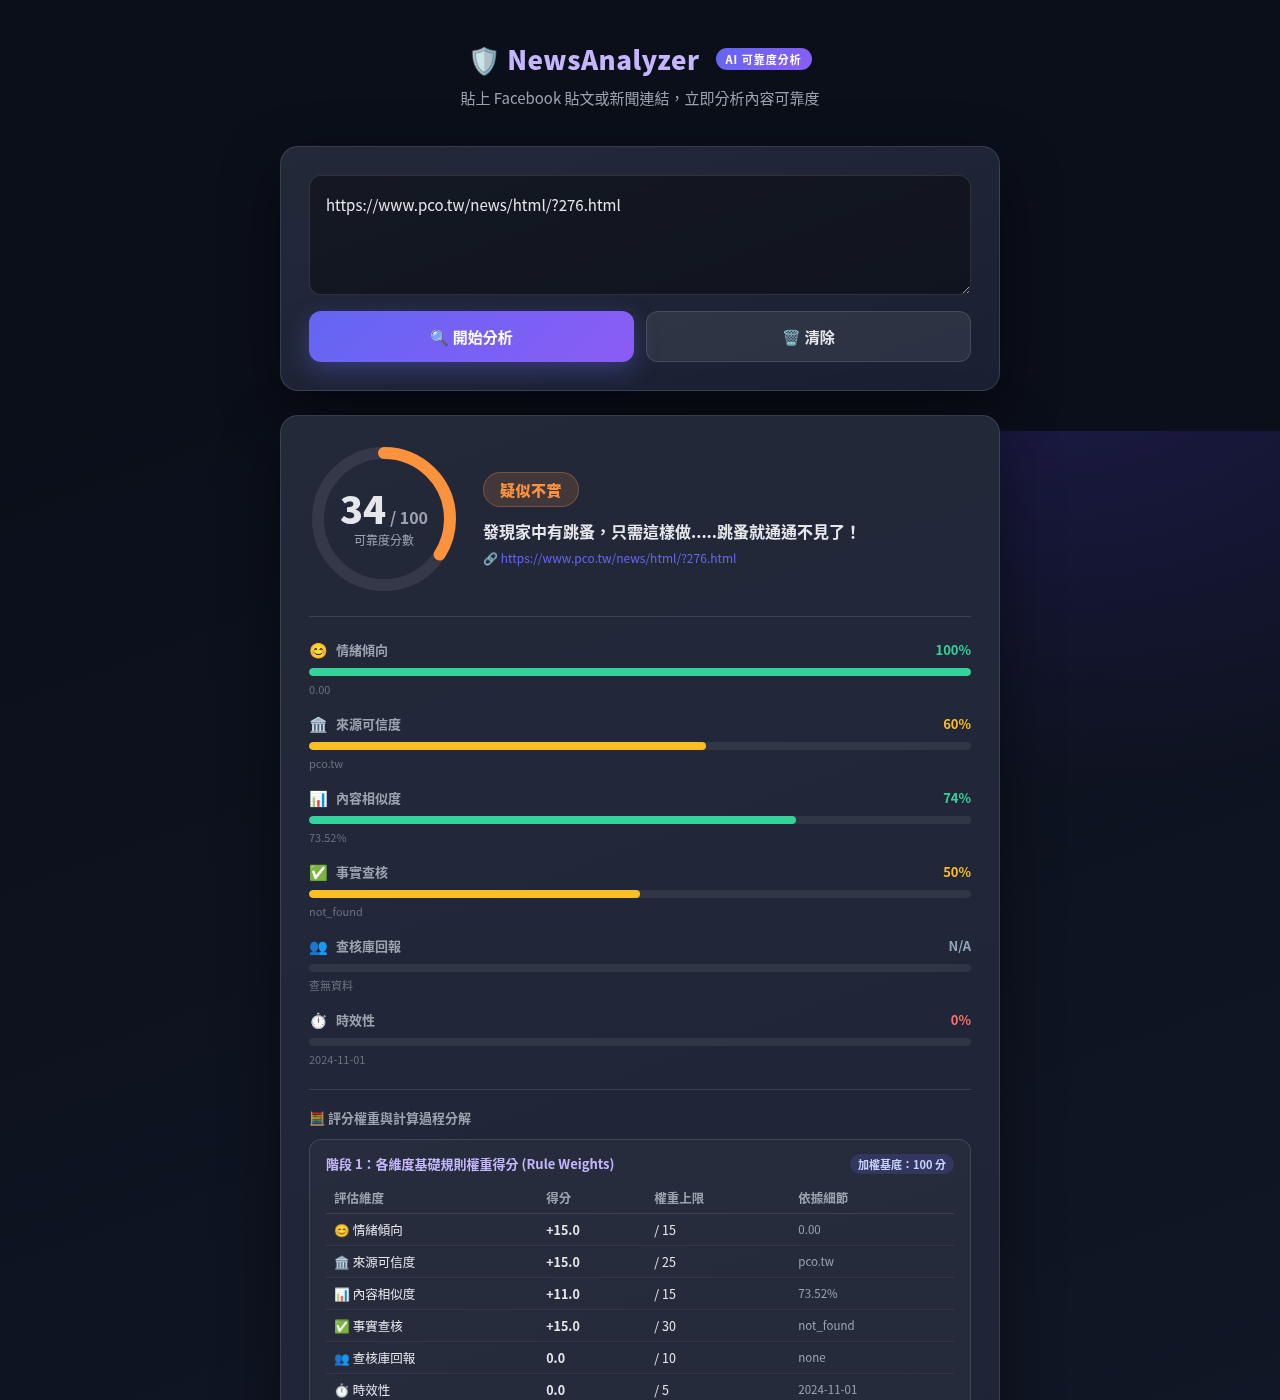
\includegraphics[width=\textwidth]{app_parsing_result_crop.png}
\caption{The web-based testing interface of the NewsAnalyzer backend, displaying real-time DOM parsing results, multi-signal metadata scoring, and auxiliary LLM perspective extraction directly derived from a submitted content farm URL.}
\label{fig:app_parsing}
\end{figure}

Because this specific claim had no pre-existing match in Cofacts above threshold ($\theta_{\text{sim}} \ge 0.72$), the SBERT retriever returned \texttt{not\_found} (Figure~\ref{fig:app_parsing}). Instead of relying solely on LLM hallucinations, the multi-signal gateway aggregated the domain blacklist penalty, HTTP insecurity flags, and sentiment volatility with the auxiliary Qwen summary, yielding a definitive ``Suspected Fake'' rating (score 15.9).

%======================================================================
% 6 DISCUSSION
%======================================================================
\section{Discussion}

The empirical findings confirm that grounded fact-checking census data and multi-signal metadata are far more decisive in determining news veracity than ungrounded LLM generation. While large language models excel at synthesizing complex text and extracting diverse perspectives, treating them as autonomous judges introduces unacceptable risks of hallucination, temporal obsolescence, and stylistic vulnerability.

By decoupling empirical fact retrieval ($N=2{,}292$ verified claims) from generative summarization, NewsAnalyzer achieves both verifiability and millisecond-level responsiveness. The asymmetric safety anchor ($S \le 25$) guarantees that empirical counter-evidence strictly overrides generative model outputs.

Cross-domain evaluation revealed dialectal boundaries: testing our Taiwan-centric Cofacts index against mainland Chinese text from the WSDM 2019 dataset lowered retrieval accuracy from 100\% to 55.3\%, underscoring that regional linguistic nuances and political vocabularies require localized seed corpuses rather than generalized Chinese language models.

%======================================================================
% 7 CONCLUSION
%======================================================================
\section{Conclusion}

NewsAnalyzer demonstrates that robust, privacy-preserving fake news detection on Traditional Chinese social media requires shifting from brute-force LLM prompting to an empirical, multi-signal paradigm. By combining an offline macro census of 2,292 IFCN-verified Cofacts claims with a multi-attribute metadata scoring engine and local auxiliary perspective extraction, the system achieves 95.3\% accuracy ($F_1 = 0.974$) and 1.48\,ms retrieval latency on consumer hardware with zero data egress.

\section*{Reproducibility and Code Availability}
To facilitate independent replication, the evaluation datasets, benchmarking scripts, and Chrome extension source code are available at: \url{https://github.com/min20120907/NewsAnalyzer}.

%======================================================================
% REFERENCES
%======================================================================
\begin{thebibliography}{99}
\fontsize{8pt}{9.5pt}\selectfont
\setlength{\itemsep}{0pt}
\setlength{\parsep}{0pt}
\setlength{\parskip}{0pt}

\bibitem{wang2017liar}
W.~Y. Wang, ``Liar, Liar Pants on Fire: A New Benchmark Dataset for Fake News Detection,'' in \emph{Proc. ACL}, 2017, pp. 422--426.

\bibitem{guo2022survey}
Z.~Guo, M.~Schlichtkrull, and A.~Vlachos, ``A Survey on Automated Fact-Checking,'' \emph{Trans. ACL}, vol.~10, pp. 178--206, 2022.

\bibitem{Bianchi2024trustworthiness}
J.~Bianchi, M.~Pratelli, M.~Petrocchi, and F.~Pinelli, ``Evaluating Trustworthiness of Online News Publishers via Article Classification,'' in \emph{Proc. ACM SAC '24}, 2024, pp.~671--678.

\bibitem{devlin2019bert}
J.~Devlin, M.-W.~Chang, K.~Lee, and K.~Toutanova, ``BERT: Pre-training of Deep Bidirectional Transformers for Language Understanding,'' in \emph{Proc. NAACL-HLT}, 2019, pp. 4171--4186.

\bibitem{perez2018automatic}
V.~P{\'e}rez-Rosas, B.~Kleinberg, A.~Lefevre, and R.~Mihalcea, ``Automatic Detection of Fake News,'' in \emph{Proc. COLING}, 2018, pp. 3391--3401.

\bibitem{rashkin2017truth}
H.~Rashkin, E.~Choi, J.~Y. Jang, S.~Volkova, and Y.~Choi, ``Truth of Varying Shades: Analyzing Language in Fake News and Political Fact-Checking,'' in \emph{Proc. EMNLP}, 2017, pp. 2931--2937.

\bibitem{potthast2018stylometric}
M.~Potthast, J.~Kiesel, K.~Reinartz, J.~Bevendorff, and B.~Stein, ``A Stylometric Inquiry into Hyperpartisan and Fake News,'' in \emph{Proc. ACL}, 2018, pp. 231--240.

\bibitem{pennycook2019fighting}
G.~Pennycook and D.~G. Rand, ``Fighting Misinformation on Social Media Using Crowdsourced Judgments of News Source Quality,'' \emph{Proc. Natl. Acad. Sci.}, vol. 116, no.~7, pp. 2521--2526, 2019.

\bibitem{allen2021scaling}
J.~Allen, A.~A. Arechar, G.~Pennycook, and D.~G. Rand, ``Scaling Up Fact-Checking Using the Wisdom of Crowds,'' \emph{Science Advances}, vol.~7, no.~36, p. eabf4393, 2021.

\bibitem{reimers2019sbert}
N.~Reimers and I.~Gurevych, ``Sentence-BERT: Sentence Embeddings using Siamese BERT-Networks,'' in \emph{Proc. EMNLP-IJCNLP}, 2019, pp.~3980--3990.

\bibitem{qwen2025report}
Qwen Team, ``Qwen3 Technical Report,'' arXiv preprint arXiv:2505.09388, 2025.

\bibitem{gguf2023}
G.~Gerganov, ``ggml-org/ggml: Tensor library for machine learning (GGUF),'' 2023. [Online]. Available: \url{https://github.com/ggml-org/ggml}

\bibitem{chrome_mv3}
Google Developers, ``Chrome Extensions Manifest V3 Overview,'' 2023. [Online]. Available: \url{https://developer.chrome.com/docs/extensions/develop/migrate/what-is-mv3}

\bibitem{cofacts2020}
B.~Lee, J.~Liang, and Cofacts Contributors, ``Cofacts: A Collaborative Fact-Checking System for Instant Messaging Platforms,'' \emph{g0v.tw Civic Tech Open Database}, 2020. [Online]. Available: \url{https://cofacts.tw}

\bibitem{ifcn2020}
IFCN, ``The IFCN Code of Principles,'' \emph{Poynter Institute}, 2020. [Online]. Available: \url{https://ifcncodeofprinciples.poynter.org/}

\bibitem{tfc2023}
Taiwan FactCheck Center, ``Fact-Checking Methodologies and Verified Public Archives,'' 2023. [Online]. Available: \url{https://tfc-taiwan.org.tw}

\bibitem{lim2023factchecking}
G.~Lim and S.~T.~Perrault, ``Fact Checking Chatbot: A Misinformation Intervention for Instant Messaging Apps,'' in \emph{Mobile Communication in Asia} (Springer, 2023), pp.~197--224.

\bibitem{vu2024freshllms}
T.~Vu, et al., ``FreshLLMs: Refreshing Large Language Models with Search Engine Augmentation,'' in \emph{Findings of ACL}, 2024, pp.~13697--13710.

\bibitem{chern2023factool}
I.-C.~Chern, et al., ``FacTool: Factuality Detection in Generative AI,'' arXiv preprint arXiv:2307.13528, 2023.

\bibitem{hassan2017claimbuster}
N.~Hassan, et al., ``ClaimBuster: The First-Ever End-to-End Fact-Checking System,'' in \emph{Proc. ACM CSCW '17}, 2017.

\bibitem{shu2019defend}
K.~Shu, L.~Cui, S.~Wang, D.~Lee, and H.~Liu, ``dEFEND: Explainable Fake News Detection,'' in \emph{Proc. ACM KDD '19}, 2019, pp.~395--405.

\end{thebibliography}

\end{document}
